\documentclass[tikz,border=10pt]{standalone}
\usepackage{tikz}
\begin{document}
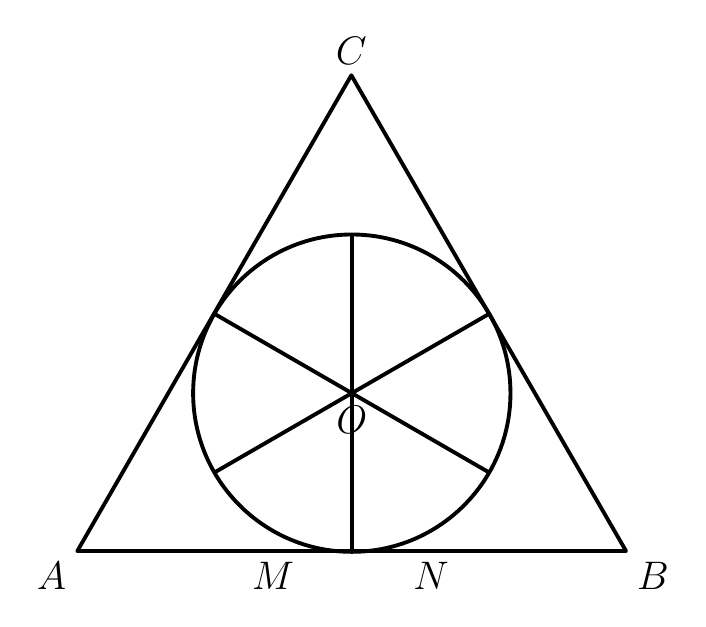
\begin{tikzpicture}[line join=round, line width=1.4pt]
% Coordinates: x = px*s, y = (487-py)*s, s = 0.017021 cm
\coordinate (C) at (4.620,7.182);
\coordinate (A) at (1.140,1.140);
\coordinate (B) at (8.109,1.140);
\coordinate (O) at (4.626,3.145);
\coordinate (M) at (3.626,1.140);
\coordinate (N) at (5.634,1.140);
\coordinate (T) at (4.626,1.140);   % foot of incircle on AB
% Incircle radius 118.4 px = 2.015 cm; endpoints on the circle
\coordinate (Vt) at (4.626,5.160);  % circle top (y = O + r)
\coordinate (D1a) at (2.881,4.153); % 150 deg, upper-left
\coordinate (D1b) at (6.371,2.137); % 330 deg, lower-right
\coordinate (D2a) at (2.881,2.137); % 210 deg, lower-left
\coordinate (D2b) at (6.371,4.153); % 30 deg, upper-right

% Triangle
\draw (A) -- (C) -- (B) -- cycle;

% Incircle (full circle)
\draw (O) circle[radius=2.015];

% Interior segments (trimmed to the incircle)
\draw (Vt) -- (T);
\draw (D1a) -- (D1b);
\draw (D2a) -- (D2b);

% Labels
\node[above] at (C) {\fontsize{13.5}{16.2}\selectfont $C$};
\node[below left] at (A) {\fontsize{13.5}{16.2}\selectfont $A$};
\node[below right] at (B) {\fontsize{13.5}{16.2}\selectfont $B$};
\node at (4.626,2.808) {\fontsize{13.5}{16.2}\selectfont $O$};
\node[below] at (M) {\fontsize{13.5}{16.2}\selectfont $M$};
\node[below] at (N) {\fontsize{13.5}{16.2}\selectfont $N$};
\end{tikzpicture}
\end{document}